
\documentclass[12pt]{article}   % list options between brackets
\usepackage{graphicx}
\usepackage{subfigure}

% type user-defined commands here

\begin{document}

\title{CS288 Assignment 3: Word Alignment}   % type title between braces
\author{Reynold Shi Xin}         % type author(s) between braces
\date{rxin@cs.berkeley.edu}    % type date between braces
\maketitle

%%%%%%%%%%%%%%%%%%%%%%%%%%%%%%%%%%%%%%%%%%%%%%%%%%%%%%%%%%%%%%%%%%%%%%%
%%%%%%%%%%%%%%%%%%%%%%%%%%%%%%%%%%%%%%%%%%%%%%%%%%%%%%%%%%%%%%%%%%%%%%%
\begin{abstract}
We have implemented three models for word alignment in statistical translation: a naive heuristic model of choice, the IBM Model 1, and the HMM model proposed by Vogel. We examine algorithmic trade-offs in implementation and assess the three models using the Alignment Error Rate and the BLEU score produced by the translation. The two statistical models produce better results than the heuristic model, and the HMM model produces the best AER and BLEU score.
\end{abstract}


%%%%%%%%%%%%%%%%%%%%%%%%%%%%%%%%%%%%%%%%%%%%%%%%%%%%%%%%%%%%%%%%%%%%%%%%%%%%%%
%%%%%%%%%%%%%%%%%%%%%%%%%%%%%%%%%%%%%%%%%%%%%%%%%%%%%%%%%%%%%%%%%%%%%%%%%%%%%%
\section{Alignment Models}

We have implemented three alignment models: a heuristic model, an IBM-Model-1-based model \cite{ibm-models}, and an HMM-based model as proposed in \cite{hmm-model}.

\subsection{Heuristic Model}
Given an English word $e$, the heuristic model simply aligns the English word to a French word by:
$$ \arg\max_f \frac{c(f,e)}{c(e) \cdot c(f)} $$
where $c(f,e)$ is the number of times $f$ and $e$ appear together in a sentence pair.

In reality, it is possible for an English word to be not aligned with any of the French words, also known as null alignment. This model does not take null alignment into account.


\subsection{IBM Model 1}
\label{sec:em}

The IBM Model 1 is a mixture-based model proposed by Brown et al.~in \cite{ibm-models}. In this model, the probability of an alignment $a$ for a sentence pair $(\mathbf{f}, \mathbf{e})$ is the product of the alignment probability and the summation probability:
$$ P(\mathbf{f}, a|\mathbf{e}) = \prod_{i} P(a_i = j|i, |\mathbf{e}|, |\mathbf{f}|) \cdot P(\mathbf{f}_i|\mathbf{e}_j) $$
where the alignment probability is evenly distributed among all positions:
$$ P(a_i = j|i, |\mathbf{e}|, |\mathbf{f}|) = \frac{1}{|\mathbf{e}| + 1} $$

In practice, a small portion of the alignment probability is reserved for null alignment, known as the \emph{null likelihood}. In Section \ref{sec:exp}, we discuss the effect of null likelihood on the quality of the translation model.

In general, the \emph{Soft EM} algorithm is used to compute this model iteratively. In the E step, we align the sentences using the given translation prior. In the M step, we count the total posterior probability each French word is aligned to each English word. This posterior gives us a new estimate of the translation probabilities $P(f|e)$.

In \emph{Hard EM}, we do not do partial counts of probability. Rather, we pick the pair of French word and English word that generates the highest likelihood, and increment the posterior count by one for that pair. Hard EM uses less memory due to the more sparse translation matrix, and also converges faster. It however produces lower quality than Soft EM because of the information loss between iterations.

When implementing Soft EM, we accidentally introduced a bug in the alignment probability model that slightly improved the quality of the Soft EM algorithm. In this \emph{Weird Soft EM} model, null likelihood is inflated during learning phase. But once learning is completed, the null likelihood returns to its original value.

In Section \ref{sec:exp}, we compare the quality of alignments produced by these three variants of IBM Model 1.


\subsection{HMM Model}
IBM Model 1 assumes each position is equally likely in alignment. Most natural languages, however, have a strong localization effect that words do not distribute arbitrarily over sentence positions \cite{hmm-model}. The HMM model assumes a first-order dependence on the alignment position, i.e. a word's alignment position depends on that of the previous word, as shown in Figure \ref{fig:hmm}.

\begin{figure}[h*]
	\centering
	\includegraphics[width=0.7\linewidth]{hmm.png}
	\label{fig:hmm}
	\caption{Graphical model for HMM alignment.}
\end{figure}

Statistically, the HMM model can be expressed as
$$ P(f,a|e) = \prod_j P(a_j|a_{j-1}) \cdot P(f_j|e_i) $$
where $P(a_j|a_{j-1})$ is the transition probability and $P(f_j|e_i)$ is the emission probability in HMM.

The Soft EM algorithm mentioned in the previous subsection is employed to train the HMM model. In each iteration, we use the forward-backward algorithm \cite{forward-backward} to calculate the posterior.


%%%%%%%%%%%%%%%%%%%%%%%%%%%%%%%%%%%%%%%%%%%%%%%%%%%%%%%%%%%%%%%%%%%%%%%%%%%%%%
%%%%%%%%%%%%%%%%%%%%%%%%%%%%%%%%%%%%%%%%%%%%%%%%%%%%%%%%%%%%%%%%%%%%%%%%%%%%%%
\section{Experiments}
\label{sec:exp}


\subsection{The corpus}

\begin{table}
\centering
\begin{tabular}{ c | c | c  }
	Num. Sentences & French Voc. Size & English Voc. Size \\
	\hline
	100 & 2145 & 1902 \\
	1000 & 4253 & 3663 \\
	10,000 & 12957 & 10363 \\
	100,000 & 33709 & 25894 \\
	1,000,000 & 82251 & 64660 \\
\end{tabular}
\caption{Vocabulary size of the corpus.}
\label{tbl:corpus}
\end{table}

The models were trained using a collection of French-English transcripts of the Canadian parliamentary proceedings. The corpus contains a total of one million pairs of sentences. Table \ref{tbl:corpus} shows the size of the vocabulary contained in this corpus.

For testing purpose, the sentences have also been hand-aligned. We report the Alignment Error Rate, or AER, produced by the different models. For comparing the quality of alignment among the three models, we used the alignment outputs to extract phrase tables and test the translation results produced by a phrase-based decoder. The translation test harness uses the same data as the aligner's input, and reports the BLEU scores.


\begin{figure}[h*]
\centering
\subfigure[Comparison of three EM methods.]{
	\includegraphics[height=0.47\linewidth, angle=-90]{graphs/em.eps}
	\label{fig:em}
}
\subfigure[Null Likelihood.]{
	\includegraphics[height=0.47\linewidth, angle=-90]{graphs/null.eps}
	\label{fig:null}
}
\label{fig:params}
\caption{EM and null alignment likelihood.}
\end{figure}


\subsection{Variants of EM algorithms for IBM Model 1}
Figure \ref{fig:em} shows how the three variants of the EM algorithm perform with respect to AER. The Hard EM variant ran for 10 iterations, while the two soft EM variants ran for 30 iterations.

When there were little data, the Hard EM algorithm performed the worst and the Weird Soft EM algorithm was the clear choice. However, as the corpus size grows, the difference between Soft EM and Weird Soft EM diminished, eventually resulting in less than one percent difference between the two.


\subsection{Null Likelihood}
We also studied the effect of the null alignment likelihood in the context of IBM Model 1. Holding everything constant, we varied the null likelihood from $0.1$ to $0.35$ and trained the aligner using the Soft EM algorithm. 

Figure \ref{fig:null} reports the results. Although we were able to find a sweet spot at 0.28, the null likelihood has a rather small effect on the AER. It merely affects AER by less than one percent.


\subsection{Alignment Quality and Error Analysis}

\begin{figure}[h*]
\centering
\subfigure[]{
	\includegraphics[height=0.7\linewidth, angle=-90]{graphs/perf_aer.eps}
	\label{fig:aer}
}
\subfigure[.]{
	\includegraphics[height=0.7\linewidth, angle=-90]{graphs/perf_bleu.eps}
	\label{fig:bleu}
}
\label{fig:perf}
\caption{Alignment quality of three models.}
\end{figure}

We ran the three models (Heuristic, IBM Model 1 with Weird Soft EM, and HMM) on the corpus up to 1 million sentence pairs. The general trend for all models is that both AER and BLEU score improves significantly as we use a larger corpus. This confirms the hypothesis in \cite{data-effect}. Even in the simple Heuristic model, AER was reduced to 46\% and BLEU was at 21.2 with a million sentences. IBM Model 1 produced an AER of 23\% and BLEU score of 25.8. The HMM model performed the best, with an AER of 16\% and BLEU of 28.8.

Having examined the alignment output by each of the model, we outline the weakness of the models here.

The Heuristic model aligns English words to French words. Aside from the fact that the Heuristic model is naive, many French words are not aligned at all to anything because the French sentences are in general longer than the English translations.

For IBM Model 1, we observe the well-known problem that French words are more likely to be aligned to rare English words. As shown in Figure \ref{fig:model1align}, four French words are aligned to the English word ``Canadair''. 

\begin{figure}[h]
\centering
{\tiny
\begin{verbatim}
	[#]                                             | cela
	   ( )   ( )                      #             | �quivaut
	      ( )    #                                  | �
	      (#)                                       | peu
	      (#)                                       | pr�s
	            [#]                                 | �
	               [ ]                              | les
	                     [#]                        | 440
	                        [#]                     | millions
	                  ( )   ( )                     | de
	                  [#]                           | dollars
	                           [ ]    #             | vers�s
	             #                [ ]               | �
	                                 [#]            | Canadair
	                                    (#)         | en
	                #                   ( )         | le
	                                  # ( )         | espace
	                                    ( )         | de
	                                       [#]      | deux
	                                          [#]   | ans
	                                             [#]| .
	------------------------------------------------'
	 t  i  r  e  t  t  $  4  m  p  t  C  i  t  y  . 
	 h  s  o  q  o  h     4  i  a  o  a  n  w  e    
	 a     u  u     e     0  l  i     n     o  a    
	 t     g  a              l  d     a        r    
	       h  l              i        d        s    
	       l                 o        a             
	       y                 n        i             
	                                  r
\end{verbatim}
}
\label{fig:model1align}
\caption{An example alignment for IBM Model 1.}
\end{figure}

For both the HMM model and the IBM model, we are doing one-way alignment from French to English. This rules out the possibility that multiple English words being aligned to a single French word. To overcome this problem, Liang proposed in \cite{align-agreement} using an agreement model that does bi-directional alignment based on two one-way alignments. 
